\documentclass[10pt,a4paper]{article}

\usepackage[a4paper,top=1.7cm,bottom=1.7cm,left=1.75cm,right=1.75cm]{geometry}
\usepackage{fontspec}
\usepackage[french]{babel}
\usepackage[hidelinks]{hyperref}
\usepackage{xcolor}
\usepackage{graphicx}
\usepackage{titlesec}
\usepackage{enumitem}

\setmainfont[Scale=1.04]{Arial}
\pagestyle{empty}
\setlength{\parindent}{0pt}
\setlength{\parskip}{1pt}
\linespread{1.04}
\setlist[itemize]{leftmargin=1.25em,itemsep=3pt,topsep=4pt,parsep=0pt}

\definecolor{heading}{HTML}{123867}
\titleformat{\section}{\large\bfseries\color{heading}}{}{0pt}{}[\vspace{-5pt}\rule{\linewidth}{0.5pt}]
\titlespacing{\section}{0pt}{12pt}{7pt}

\newcommand{\entryspace}{\vspace{5pt}}

\newif\ifwithphoto
\withphotofalse
\IfFileExists{with_photo.flag}{\withphototrue}{}

\newcommand{\role}[3]{%
  \textbf{#1} \hfill #3\\
  \textit{#2}\vspace{1pt}
}

\newcommand{\edu}[4]{%
  \textbf{#1} -- #2 \hfill #3 #4\\[3pt]
}

\begin{document}

\ifwithphoto
\begin{minipage}[c]{0.76\linewidth}
{\LARGE \textbf{Kossi Richard Allado}}\\
\textbf{Etudiant ingenieur en Cybersecurite et Intelligence Artificielle}\\
Beni Mellal, Maroc | +212 621 074 305 | \href{mailto:alladokossirichard2025@gmail.com}{alladokossirichard2025@gmail.com}\\
\href{https://allakori.github.io/}{allakori.github.io} | \href{https://github.com/ALLAKORI}{github.com/ALLAKORI} | \href{https://www.linkedin.com/in/kossi-richard-allado-50177b2a5}{linkedin.com/in/kossi-richard-allado}
\end{minipage}
\hfill
\begin{minipage}[c]{0.18\linewidth}
\raggedleft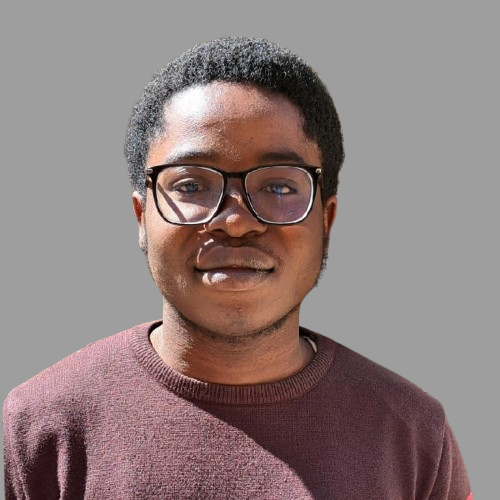
\includegraphics[width=2.35cm]{photo_richard.png}
\end{minipage}
\else
{\LARGE \textbf{Kossi Richard Allado}}\\
\textbf{Etudiant ingenieur en Cybersecurite et Intelligence Artificielle}\\
Beni Mellal, Maroc | +212 621 074 305 | \href{mailto:alladokossirichard2025@gmail.com}{alladokossirichard2025@gmail.com}\\
\href{https://allakori.github.io/}{allakori.github.io} | \href{https://github.com/ALLAKORI}{github.com/ALLAKORI} | \href{https://www.linkedin.com/in/kossi-richard-allado-50177b2a5}{linkedin.com/in/kossi-richard-allado}
\fi

\section{Profil}
Etudiant ingenieur en cybersecurite et IA a l'ENSA Beni Mellal, avec une orientation principale vers la securite offensive, le pentest et la securite applicative. Experience pratique a travers des labs et CTF : reconnaissance, web security, IAM avec Keycloak, PKI/OpenSSL, Linux hardening, investigation de logs, forensic et documentation technique. Recherche un stage PFA en cybersecurite a partir de juillet 2026, avec un interet particulier pour la securisation des identites, des applications et des systemes d'information.

\section{Competences techniques}
\textbf{IAM / PKI / Systemes :} Keycloak, MFA/TOTP, RBAC, OpenSSL, PKI, Linux, SELinux, AppArmor, Lynis, SSH.\\
\textbf{Securite offensive / applicative :} Kali Linux, Nmap, Wireshark, Burp Suite, Hydra, reconnaissance, SQL injection, XSS, CTF.\\
\textbf{SOC / Detection / DFIR :} Splunk, Windows logs, Linux logs, auditd, IOC, timeline, Volatility, WinPMEM, Autopsy, FTK Imager.\\
\textbf{Programmation :} Python, Bash, C, SQL, Git/GitHub, Pandas, Scikit-learn, Jupyter.

\section{Projets techniques}
\textbf{Investigation SOC/DFIR d'une intrusion type Volt Typhoon} \hfill 2026\\
\href{https://allakori.github.io/writeups/tryhackme/volt-typhoon/}{Write-up technique}
\begin{itemize}
  \item Investigation DFIR d'une intrusion type APT avec Splunk : acces initial, execution WMIC/PowerShell, persistance web shell, credential access, C2 et effacement de traces.
  \item Correlation d'evenements Windows et applicatifs pour produire une timeline, identifier les IOC, mapper les actions sur MITRE ATT\&CK et documenter les preuves exploitables.
\end{itemize}
\entryspace

\textbf{Analyse forensic disque et memoire pour reponse a incident} \hfill 2026\\
\href{https://github.com/ALLAKORI/linux-security-labs}{github.com/ALLAKORI/linux-security-labs}
\begin{itemize}
  \item Conduite d'une analyse forensic disque/memoire avec WinPMEM, Volatility, Autopsy et FTK Imager afin d'extraire processus, connexions reseau, artefacts systeme et traces utilisateur.
  \item Structuration d'un rapport d'incident : hypotheses, methodologie, timeline, artefacts observes, interpretation des resultats et recommandations de remediation.
\end{itemize}
\entryspace

\textbf{Plateforme IAM, PKI et securite applicative} \hfill 2025\\
\href{https://github.com/ALLAKORI/cybersecurity-iam-labs}{github.com/ALLAKORI/cybersecurity-iam-labs}
\begin{itemize}
  \item Deploiement d'un environnement IAM avec Keycloak : realms, utilisateurs, roles, MFA/TOTP, RBAC et tests de controle d'acces.
  \item Mise en pratique OpenSSL/PKI et tests DVWA sur SQL injection/XSS, avec analyse des causes et redaction de contre-mesures applicatives.
\end{itemize}
\entryspace

\textbf{Competition CSIA CTF 2026 - 1ere place avec Team GHOSTSHELL} \hfill 2026\\
\href{https://github.com/ALLAKORI/csia-ctf-2026-writeups}{github.com/ALLAKORI/csia-ctf-2026-writeups}
\begin{itemize}
  \item Participation en equipe et obtention de la 1ere place ; resolution de challenges web, steganographie, OSINT, forensic et misc sous contrainte de temps.
  \item Redaction de write-ups reproductibles mettant en avant l'enumeration, les hypotheses, les commandes utilisees, les preuves et le raisonnement de resolution.
\end{itemize}
\entryspace

\section{Experience}
\role{Stagiaire IA / Maintenance predictive}{ONEE - Branche Eau, Kasba Tadla}{Aout 2025}
\begin{itemize}
  \item Preparation de donnees capteurs et prediction de defauts de pompes haute pression.
  \item Prototype Python avec Random Forest, Pandas, Scikit-learn et interface de test.
\end{itemize}

\section{Formation}
\edu{Cycle ingenieur}{Cybersecurite et Intelligence Artificielle, ENSA Beni Mellal}{2024 - Present}{}
\edu{DEUST}{Mathematiques, Informatique, Physique, FST Fes}{2022 - 2024}{-- Mention Bien}
\edu{Baccalaureat scientifique}{Serie D, Lycee de Djagble, Togo}{2022}{-- Mention Tres Bien}

\section{Certifications}
Cisco Ethical Hacker | TryHackMe Junior Penetration Tester Learning Path (en cours, finalisation prevue mai 2026) | Google Cybersecurity : Foundations et Play It Safe | TryHackMe Advent of Cyber 2025 | Udemy Cryptography and Hashing

\section{Langues}
Francais : courant | Anglais : professionnel technique | Ewe : langue maternelle

\section{Centres d'interet}
CTF cybersecurite : participation a des challenges et redaction de write-ups | Veille technologique : cybersecurite, IA, SOC/DFIR et securite applicative | Piano : pratique musicale reguliere

\end{document}
